% Created by Dan O'Shea (@djoshea) 2022.
% Inspired by https://www.nature.com/nature-index/news-blog/researchers-embracing-visual-tools-contribution-matrix-give-fair-credit-authors-scientific-papers

\documentclass[margin=1mm]{standalone}
\PassOptionsToPackage{svgnames}{xcolor}
\usepackage{tikz} 
\usetikzlibrary{calc,intersections}

\usepackage{libertine}

\tikzset{
    tile/.style = {
        align=center,
        minimum size=6mm,
        anchor=north west,
    },
    col header/.style={
        tile,
        anchor=north west,
        yshift=-1mm,
        rotate=45,
        inner sep=0,
        outer sep=0,
    },
    row label/.style={
        tile,
        anchor=north east,
        inner sep=0,
        outer sep=0,
        xshift=3mm,
    },
    legend line/.style={
        anchor=north west,
        inner xsep=0,
        inner ysep=2mm,
        outer sep=0,
    },
}

% define the intensity levels here
\def\hi{100}
\def\mid{50}
\def\lo{20}

% and the 100% intensity color here, which will blended to white
\colorlet{tilecolor}{Orchid}

\begin{document}
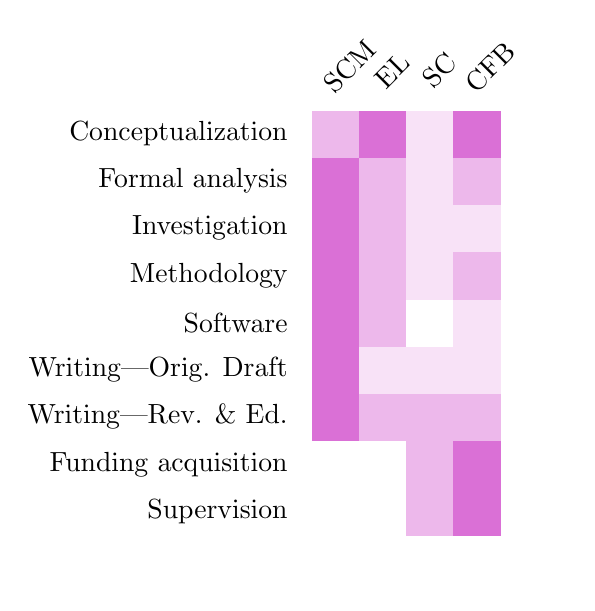
\begin{tikzpicture}[scale=0.6]

% column labels
\foreach \a [count=\n] in {
    SCM,    % Stewart Charles McDowall
    EL,     % Elizabeth Lanphear
    SC,      % Stefano Cucurachi
    CFB,    % Carlos Felipe Blanco
    % ... (other authors, if any)
} {
    \node[col header] at (\n,0) {\a};
}

% row labels
\foreach \a [count=\i] in {
    Conceptualization,
    Formal analysis,
    Investigation,
    Methodology,
    % Resources,
    Software,
    Writing---Orig. Draft,
    Writing---Rev. \& Ed.,
    Funding acquisition,
    Supervision,
} {
    \node[row label] at (0,-\i) {\a};
}

\foreach \y [count=\n] in {
    % Intensity levels for each row label for SCM, LL, SC, CFRB...
    % The intensity values (\hi, \mid, \lo, 0) should correspond to the level of contribution in the order of authors listed above
    {\mid,\hi,\lo,\hi}, % Conceptualization
    {\hi,\mid,\lo,\mid},      % Formal analysis
    {\hi,\mid,\lo,\lo},        % Investigation
    {\hi,\mid,\lo,\mid},      % Methodology
    % {0,0,\mid,\hi},          % Resources (none specified)
    {\hi,\mid,0,\lo},      % Software
    {\hi,\lo,\lo,\lo},        % Writing---Original Draft
    {\hi,\mid,\mid,\mid},  % Writing---Reviewing and Editing
    {0,0,\mid,\hi},      % Funding acquisition
    {0,0,\mid,\hi},      % Supervision
} {
    % heatmap tiles
    \foreach \x [count=\m] in \y {
        \node[fill=tilecolor!\x!white, tile, text=white] (tile) at (\m,-\n) {};
    }
}

    % description below heatmap 
    % \node [legend line] at (1, 0 |- tile.south) {*, $^\dagger$ these authors contributed equally};

\end{tikzpicture}
\end{document}